\documentclass[times, utf8, zavrsni, numeric]{fer}
\usepackage{booktabs}
\usepackage{graphicx}
\usepackage{subcaption}

\begin{document}

\thesisnumber{5187}
\title{Ekstrakcija tablica na skeniranim dokumentima}
\author{Kristijan Vulinović}

\maketitle

% Ispis stranice s napomenom o umetanju izvornika rada. Uklonite naredbu \izvornik ako želite izbaciti tu stranicu.
\izvornik

% Dodavanje zahvale ili prazne stranice. Ako ne želite dodati zahvalu, naredbu ostavite radi prazne stranice.
\zahvala{Zahvaljujem svima onima koji su odvojili dio svojeg vremena na ispunjavanje primjeraka tablica, kao i svima koji su pomogli prilikom prikupljanja istih.}

\tableofcontents

\chapter{Uvod}
U današnje vrijeme postoje izuzetno velike količine papirnatih dokumenata.
Samo u Sjedinjenim Američkim Državama nastaje više od milijarde novih papirnatih dokumenata svakog radnog dana. 
Mogućnost digitalizacije takvih dokumenata može biti od velike koristi prilikom pohrane, slanja ili pretraživanja istih. \cite{article:Skew-detection}
Digitalizaciju dokumenata možemo podijeliti u dva dijela: prepoznavanje teksta te prepoznavanje grafičkih objekata. \cite{conference:DetectionOfTableStructure} 
Za prepoznavanje teksta dostupan je velik broj alata koji omogućuju optičko prepoznavanje znakova (engl. \textit{optical character recognition}).
Prepoznavanje grafičkih objekata dokumenta mnogo je manje zastupljeno u odnosu na prepoznavanje teksta te je postalo popularnije tek u novije vrijeme. 
U to spada prepoznavanje linija, oblika, slika, simbola, tablica i raznih drugih objekata koji se mogu nalaziti na skeniranim dokumentima.
Najveći razvoj ovoga područja nastupio je zahvaljujući razvoju dubokih neuronskih mreža i sklopovlja koje omogućuje velike brzine izračuna koje prije nisu bile moguće.\\

Ovaj rad se fokusira isključivo na prepoznavanje tablica, što je prethodno već opisano u radovima poput \cite{conference:DetectionOfTableStructure} i \cite{conference:AutomaticTableDetectionInDocumentImages}. 
Taj postupak se dijeli na prepoznavanje položaja tablice u odnosu na ostatak dokumenta, prilikom čega je potrebno u dokumentu izdvojiti tablicu od ostatka teksta i ostalih grafičkih objekata, a što je opisano u radu \cite{article:Medium-IndependentTableDetection}.
Nakon što je tablica pronađena određuje se njezin izgled, odnosno broj redaka i stupaca, odnosno koordinate pojedine ćelije, a što je detaljnije opisano u nastavku rada. \\

Predstavljeno rješenje počinje od slike u sivim tonovima (engl. \textit{gray-scale}), koja se binarizira kako bi se dobila slika koja se sastoji od isključivo crne i bijele boje.
Dobivena crno-bijela slika koristi se u daljnjoj obradi te se provjerava je li slika rotirana, odnosno kut rotacije iste, nakon čega se slika po potrebi rotira kako bi tablica stajala okomito.
Ovako obrađena slika koristi se dalje za detekciju tablica, postupkom koji se temelji na prepoznavanju kuteva ćelija, te kasnijoj rekonstrukciji istih a koji je detaljnije opisan u nastavku rada.


\chapter{Binarizacija slike}
Početna slika dana je kao crno-bijela slika koja sadrži $256$ nijansi sive boje, gdje je crna označena sa vrijednošću $0$, a bijela sa $255$.
Prije nego li se započne bilo kakva analiza slike, potrebno je istu binarizirati, odnosno pretvoriti u oblik koji će sadržavati isključivo crne ili bijele elemente, bez ostalih nijansi sive.
To je moguće učiniti na dva načina: korištenjem fiksno definiranog praga nakon kojega ćemo svako vrijednost proglasiti crnom, ili korištenjem adaptivne binarizacije koja se temelji na usporedbi trenutnog intenziteta sive sa intenzitetom sive u okruženju.

\section{Binarizacija fiksnim pragom}
Najjednostavniji oblik binarizacije je korištenje fiksno definiranog praga.
U tom se slučaju gleda svaki pojedini slikovnog elementa te ukoliko je njegova vrijednost manja od zadanog praga, element se postavlja na crnu boju, dok se u protivnom postavlja na bijelu.
Prednosti ove metode su izrazito jednostavna implementacija, ali i velika brzina izvođenja. 
Nedostatci se primjećuju u slučajevima lošeg ili nejednoličnog osvjetljenja gdje se događa da se neki dijelovi dokumenta u potpunosti prepoznaju kao crni, unatoč činjenici da je prethodno bilo moguće razlikovati i prepoznati pozadinu od sadržaja dokumenta.
Slika \ref{fig:threshold} prikazuje opisani problem te se na istoj može primjetiti kako je u doljnjem lijevom kutu slike tamno područje, koje nakon binarizacije postaje u potpunosti crno. 
Također se primjećuje i kako je gornji desni kut slike slabije osvjetljen, zbog čega u binariziranoj slici slova postaju tanja i slabije vidljiva.\\

\begin{figure}[th!]
    \centering
    \begin{subfigure}{.5\textwidth}
        \centering
        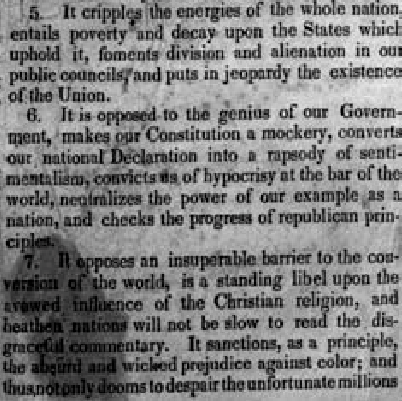
\includegraphics[width=.85\linewidth]{Images/Grayscale.png}
        \caption{Početna crno-bijela slika}
        \label{fig:sub1}
    \end{subfigure}%
    \begin{subfigure}{.5\textwidth}
        \centering
        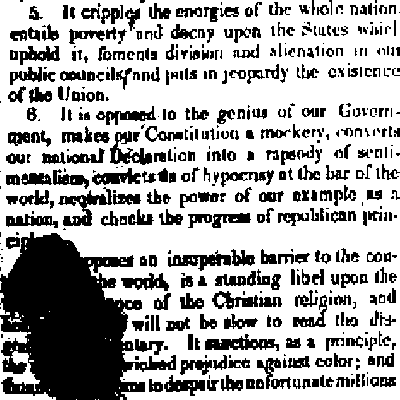
\includegraphics[width=.85\linewidth]{Images/Threshold.png}
        \caption{Slika dobivena binarizacijom fiksnim pragom}
        \label{fig:sub2}
    \end{subfigure}
    \caption{Primjer binarizacije fiksnim pragom}
    \label{fig:threshold}
\end{figure}

\section{Adaptivna binarizacija}
Problemi prikazani u prethodnom postupku rješavaju se primjenom adaptivne binarizacije koja vrijednost sakog pojedinog slikovnog elementa ne određuje samo na osnovu njegove boje, već u obzir uzima i boju okoline.
U nastavku je opisan postupak koji je predložen u \cite{AdaptiveBinarization}.
Prikazani primjeri koriste sliku \ref{fig:sub1} kao početnu.

\subsection{Filtriranje šuma}
Ovisno o stanju dokumenta i načinu digitalizacije istoga moguće je da se na dobivenoj slici pojavljuje šum, kojega je potrebno otkloniti.
Za potrebe opisanoga koristi se niskopropusni Wiener filter \cite{book:Two-Dimensional-Signal-Image-Processing}, koji se temelji na statističkoj procjeni temeljenoj na okruženju svakog pojedinog slikovnog elementa. \cite{AdaptiveBinarization}
Označimo sa $I_s(x, y)$ vrijednost slikovnog elementa početne slike, a sa $I(x, y)$ vrijednost slikovnog elementa filtrirane slike.
Tada se filtrirana slika $I$ može izračunati pomoću formule opisane u knjizi \cite{book:Two-Dimensional-Signal-Image-Processing}:
\[I(x, y) = \mu(x, y) + \frac{\sigma(x, y)^2}{(\sigma(x, y)^2 - v^2)}(I_s(x, y) - \mu(x, y))\]
Sa $\mu(x, y)$ označena je aritmetička sredina vrijednosti slikovnih elemenata u okruženju veličine $NxM$, prema formuli:
\[\mu(x, y) = \frac{1}{NM} 
    \displaystyle \sum_{i = x-\frac{N}{2}}^{x+\frac{N}{2}}
    \displaystyle \sum_{j = y-\frac{M}{2}}^{y+\frac{M}{2}}
I_s(i, j)\]
Sa $\sigma^2$ označena je varijanca vrijednosti slikovnih elemenata u okruženju veličine $NxM$, prema formuli:
\[\sigma(x, y)^2 = \frac{1}{NM} 
    \displaystyle \sum_{i = x-\frac{N}{2}}^{x+\frac{N}{2}}
    \displaystyle \sum_{j = y-\frac{M}{2}}^{y+\frac{M}{2}}
(I_s(i, j)^2 - \mu^2)\]
Sa $v^2$ je označena srednja vrijednost svih lokalnih varijanci.
Konačan rezultat filtriranja, korištenjem okruženja dimenzija $5$x$5$ prikazan je na slici \ref{fig:wiener}.

\begin{figure}[!ht]
\centering
\begin{minipage}{.5\textwidth}
    \centering
    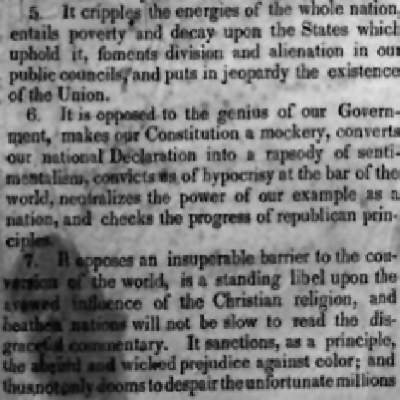
\includegraphics[width=.85\linewidth]{Images/Wiener.png}
    \caption{Slika dobivena filtriranjem šuma}
    \label{fig:wiener}
\end{minipage}%
\begin{minipage}{.5\textwidth}
    \centering
    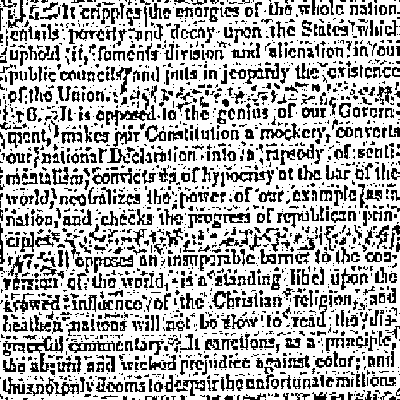
\includegraphics[width=.85\linewidth]{Images/Niblack.png}
    \captionsetup{justification=centering}
    \caption{Slika dobivena korištenjem Niblackovog algoritma adaptivne binarizacije}
    \label{fig:niblack}
\end{minipage}
\end{figure}

\subsection{Procjena sadržaja}
Sljedeći korak binarizacije temelji se na procjenjivanju sadržaja dokumenta. 
Cilj ovog koraka je procijeniti koji elementi slike pripadaju pozadini, a koji pripadaju saržaju dokumenta. 
Pritom je procijenjeni sadržaj zapravo nadskup stvarnog sadržaja, odnosno na dobivenoj slici biti će prisutan šum. 
Za potrebe ovoga koristi se Niblackov algoritam adaptivne binarizacije. \cite{AdaptiveBinarization}\\

Algoritam se temelji na ideji kliznog prozora određenih dimenzija, pomoću kojega se računa lokalni median vrijednosti $m$ te varijanca $s$. 
Kako bi se ubrzao izračun, umjesto mediana se računa aritmetička sredina $\mu$.
Konačan prag binarizacije, $T$, određuje se kao:
\[ T = m + ks \]
gdje je $k$ proizvoljna konstanta koja određuje koliko će okolina trenutnog slikovnog elementa utjecati na prag binarizacije.
Korištena vrijednost je $k = -0.2$.
Konačna slika $N$, dobivena je od početne slike $I$ na sljedeći način:
\[
    N(x, y) =
    \begin{cases}
        1,   & \quad \text{ako je } I(x, y) > T\\
        0,  & \quad \text{inače}\\
    \end{cases}
\]
Rezultati ovog postupka, korištenjem kliznog prozora dimenzija $20$x$20$, uz $k=-0.2$, prikazan je na slici \ref{fig:niblack}.
Na slici se primjećuje kako je sav tekst prepoznat i prikazan crnom bojom, ali je također prisutan i jako izražen šum.

\subsection{Procjena pozadine}
U ovom koraku pokušava se procijeniti izgled pozadine dokumenta, što je označeno sa $B$. 
Za potrebe toga koristi se obrađena početna slika $I$ te prethodno dobivena slika $N$.
Ako je neki slikovni element na slici $N$ označen nulom, taj element predstavlja pozadinu slike i njegova vrijednost na slici $B$ biti će jednaka onoj sa slike $I$.
U protivnome će vrijednost tog slikovnog elementa biti određena interpolacijom vrijednosti susjednih slikovnih elemenata.
Konačna formula za elemente slike $B$ glasi:
\[
    B(x, y) =
    \begin{cases}
        \hfil
        I(x, y),    & \quad \text{ako je } N(x, y) = 0\\[1em]
        \frac{
            \displaystyle \sum_{i = x-dx}^{x+dx}
            \displaystyle \sum_{j = y-dy}^{y+dy}
            (I(i, j)(1 - N(i, j)))
        } {
            \displaystyle \sum_{i = x-dx}^{x+dx}
            \displaystyle \sum_{j = y-dy}^{y+dy}
            (1 - N(i, j))
        }, & \quad \text{ako je} N(x, y) = 1\\

    \end{cases}
\]
Pri čemu $dx$ i $dy$ određuju dimenzije okruženja koje se gleda prilikom interpolacije.
Postupak je u cijelosti objašnjen u radu \cite{AdaptiveBinarization}.\\

\begin{figure}[!ht]
\centering
\begin{minipage}{.5\textwidth}
    \centering
    
\includegraphics[width=.85\linewidth]{Images/Background.png}
    \caption{Slika dobivena procjenom pozadine}
    \label{fig:background}
\end{minipage}%
\begin{minipage}{.5\textwidth}
    \centering
    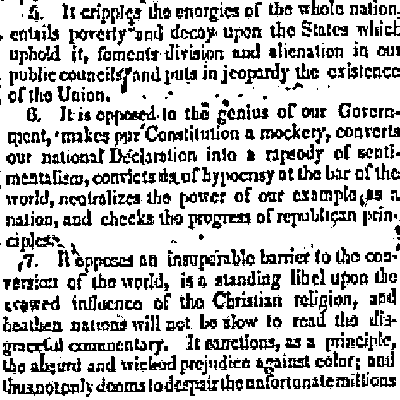
\includegraphics[width=.85\linewidth]{Images/FinalThreshold.png}
    \captionsetup{justification=centering}
    \caption{Slika dobivena binarizacijom}
    \label{fig:finalThreshold}
\end{minipage}
\end{figure}

Rezultati ovog postupka, primjenjenog na slici \ref{fig:sub1} prikazani su na slici \ref{fig:background}, uz $dx=3$ i $dy=3$.
Moguće je uočiti kako se na slici i dalje primjećuju obrisi slova, premda sama slova nisu prisutna.

\subsection{Binarizacija}
Kao što je opisano u radu \cite{AdaptiveBinarization}, u ovom koraku se provodi konačna binarizacija, uspoređivanjem izračunate pozadine $B$ i izvorne slike $I$.
Postupak se temelji na tome da je razlika u boji teksta i pozadine veća nego li razlika u boji šuma dobivenog procjenom sadržaja dokumenta i pozadine.
Ovisno o intenzitetu sive boje okruženja, računa se prag binarizacije $d$, kako bi se sačuvao tekst u tamnim područjima.
Kako bi se to postiglo, vrijednost praga $d$ mora biti manja u područjima sa tamnom pozadinom.
Konačna slika $T$ određena je formulom:
\[
    T(x, y) = 
    \begin{cases}
    1,  & \quad \text{ako je } B(x, y) - I(x, y) > d(B(x, y)) \\
    0,  & \quad \text{inače}\\
    \end{cases}
\]
Vrijednost praga, $d(B(x, y))$, moguće je procijeniti kao 
\[d = q * \delta\]
, gdje je $q$ konstanta koja je fiksno postavljena na $0.8$, a $\delta$ se računa kao razlika intenziteta sive boje na početnoj slici za mjesta koja predstavljaju pozadinu i za mjesta koja predstavljaju tekst.
Vrijednost $\delta$ možemo izračunati kao
\[
    \delta = \frac{
        \displaystyle \sum_x
        \displaystyle \sum_y
        (B(x, y) - I(x, y))
    }{
        \displaystyle \sum_x
        \displaystyle \sum_y
        N(x, y)
    }
\]

Konačan rezultat nakon primjene opisanog postupka binarizacije prikazan je na slici \ref{fig:finalThreshold}.
Za razliku od rezultata korištenjem binarizacije sa fiksnim pragom, prikazanim na slici \ref{fig:sub2}, primjećjuje se kako zatamnjeno područje u donjem lijevom kutu slike ne predstavlja problem prilikom raspoznavanja teksta od pozadine.
Također je potrebno primjetiti i šumove koji su ostali prisutni nakon trenutno opisanog postupka, a koji su riješeni u nastavku.

\subsection{Dodatna obrada slike}
Završni korak obrade slike koristi se kako bi se popravila kvaliteta konačne binarizirane slike.
Problemi koji se mogu uočiti na danim primjerima uključuju prisutnost šuma, kao i potencijalne prekide slova, gdje je moguće da neko slovo nije u potpunosti zacrnjeno.\\

\begin{figure}[!ht]
\centering
\begin{minipage}{.5\textwidth}
    \centering
    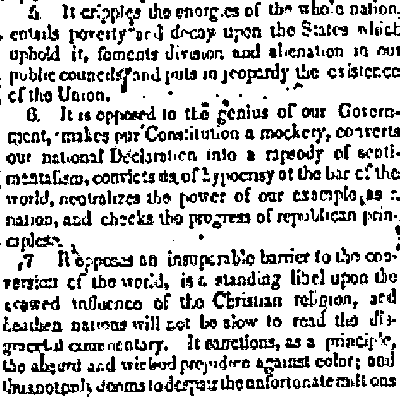
\includegraphics[width=.85\linewidth]{Images/Shrinked.png}
    \captionsetup{justification=centering}
    \caption{Slika dobivena uklanjanjem crnih slikovnih elemenata}
    \label{fig:shrink}
\end{minipage}%
\begin{minipage}{.5\textwidth}
    \centering
    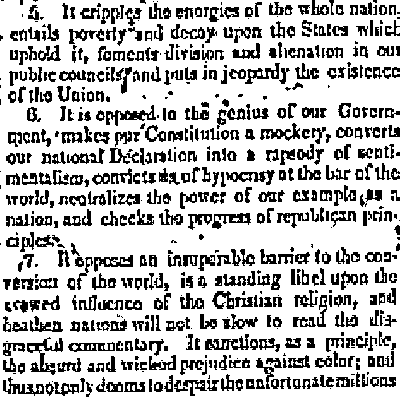
\includegraphics[width=.85\linewidth]{Images/Swell.png}
    \captionsetup{justification=centering}
    \caption{Slika dobivena uklanjanjem bijelih slikovnih elemenata}
    \label{fig:swell}
\end{minipage}
\end{figure}

Prisutnost šuma se nastoji ukloniti tako što se pregledava cijela slika te se za svaki crni slikovni element provjerava je li on rezultat šuma.
Za potrebe toga koristi se klizni prozor dimenzija $n$x$n$.
U slučaju kada je središnji element kliznog prozora crne boje, prebrojavaju se svi pozadinski (bijeli) slikovni elementi unutar kliznog prozora, što je označeno sa $P_{sh}$.
Ako je $P_{sh} > k_{sh}$, gdje je $k_{sh}$ proizvoljno zadana konstanta, središnji slikovni element se postavlja u bijelu boju.
Na slici \ref{fig:shrink} prikazan je rezultat obrade binarizirane slike navedenim postupkom uz $n = 5$ i $k_{sh} = 0.8$.
Primjećuje se kako i dalje postoje smetnje na slici, no problem nastaje kod toga što bi niža vrijednost parametra $k_{sh}$ osigurala bolje uklanjanje šumova, ali bi istovremeno povećala vjerojatnost da se uklone elementi teksta, što nije poželjno.\\

Drugi korak spomenut u ovom postupku provodi se slično kao i prethodni.
Potrebno je prebrojati broj crnih slikovnih elemenata, $P_{sw}$, koji se nalaze unutar kliznog prozora dimenzija $n$x$n$.
Ako je srednji element bijel i vrijedi $P_{sw} > k_{sw}$, središnji se element pretvara u crni.
Postupak je demonstriran na slici \ref{fig:swell}, uz $n = 5$ i $k_{sw} = 0.6$.


\chapter{Prepoznavanje zakrivljenosti slike}

\chapter{Detekcija tablice}
\section{Detekcija vrhova ćelija}
\section{Rekonstrukcija tablice}

\chapter{Primjena na automatskom prepoznavanju rukom pisanih simbola}

\chapter{Zaključak}
Zaključak.


\bibliography{literatura}
\bibliographystyle{fer}

\begin{sazetak}
Sažetak na hrvatskom jeziku.

\kljucnerijeci{Ključne riječi, odvojene zarezima.}
\end{sazetak}

\engtitle{Table Extraction on Scanned Documents}
\begin{abstract}
Abstract.

\keywords{Keywords.}
\end{abstract}

\end{document}
